\phantomsection\section*{ПРИЛОЖЕНИЕ А}\addcontentsline{toc}{section}{ПРИЛОЖЕНИЕ А}

\begin{figure}[H]
	\centering
	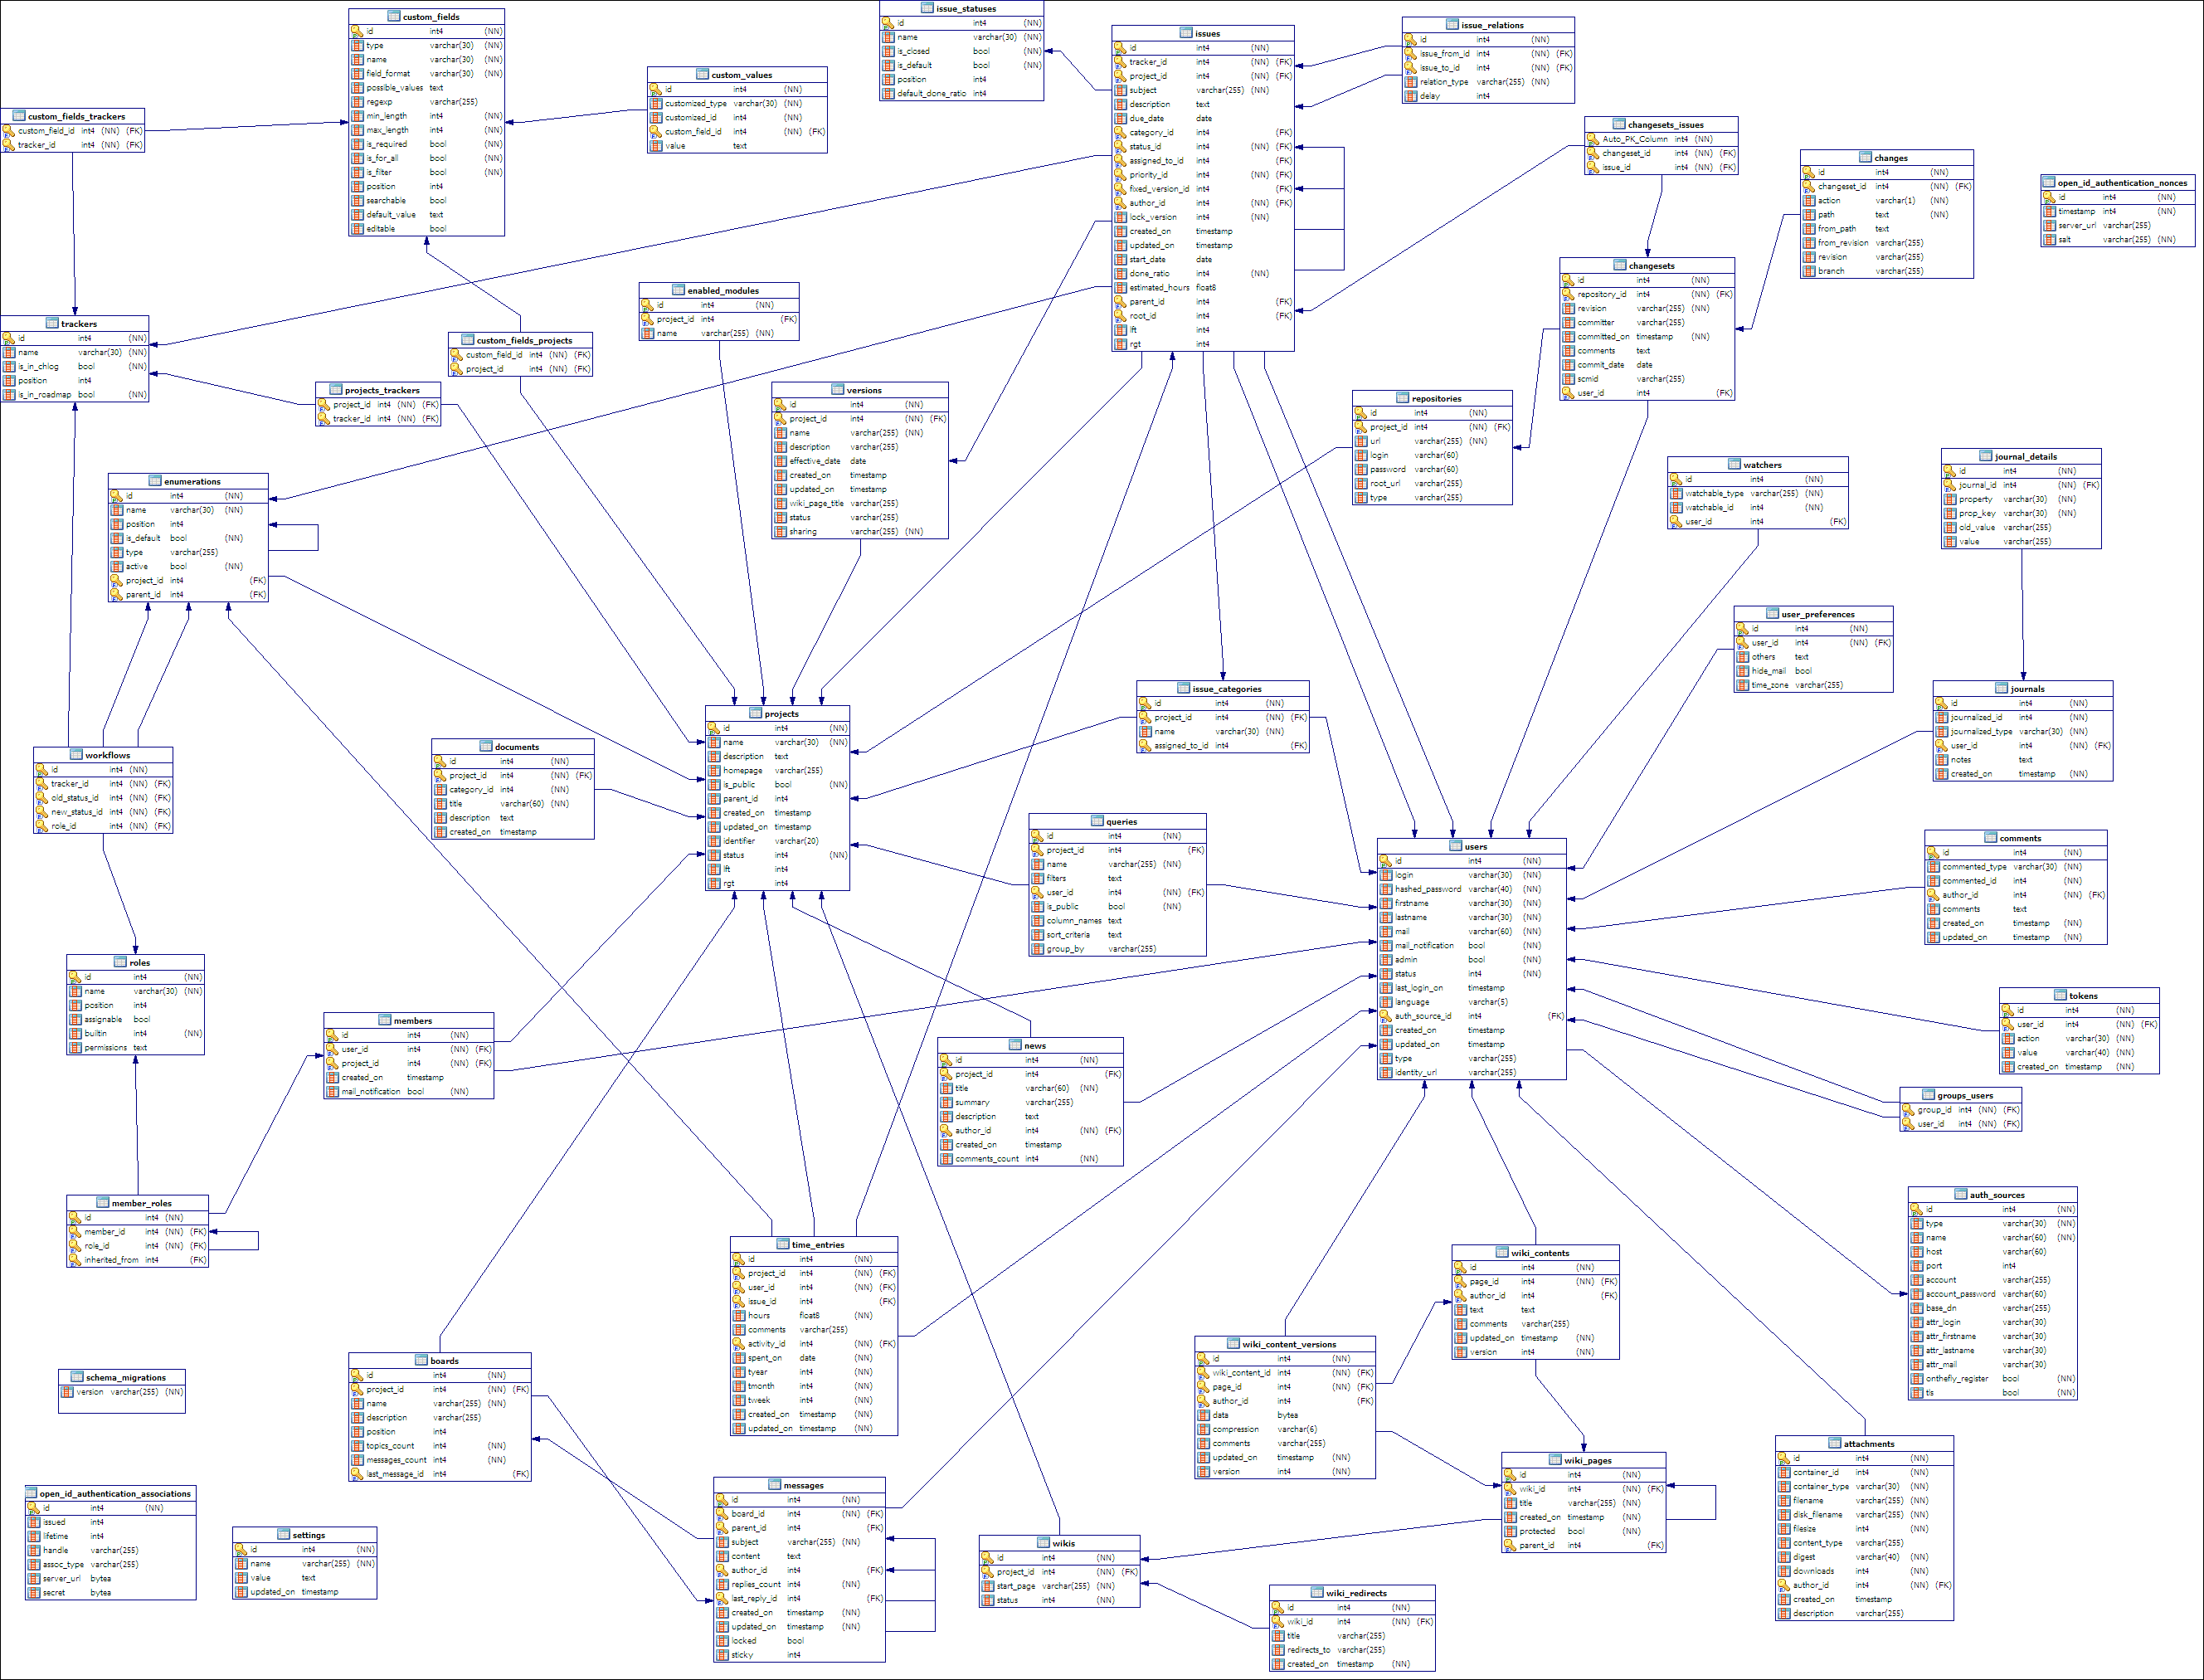
\includegraphics[width=1\textwidth]{img/redmine_er_diagram.png}
	\caption{Диаграмма базы данных сервиса redmine}
	\label{fig:redmine-er}
\end{figure}

\subsubsection{Сущность \texttt{projects}}
В системе управления проектами redmine проект является основной сущностью она содержит в себе следующую информацию:
\begin{itemize}
    \item \texttt{id} --- уникальный идентификатор проекта;
    \item \texttt{name} --- наименование проекта;
    \item \texttt{description} --- текстовое описание проекта;
    \item \texttt{homepage} --- URL домашней страницы проекта;
    \item \texttt{is\_public} --- флаг публичности проекта;
    \item \texttt{parent\_id} --- идентификатор родительского проекта;
    \item \texttt{created\_on} и \texttt{updated\_on} --- временные метки;
    \item \texttt{status} --- статус проекта (активен/архивирован);
\end{itemize}

Благодаря полю \texttt{parent\_id}, появляется возможность создавать иерархию проектов.

\subsubsection{Сущность \texttt{users}}

Таблица \texttt{users} хранит информацию о пользователях системы, и содержит в себе следующие поля:
\begin{itemize}
    \item \texttt{id} --- уникальный идентификатор пользователя;
    \item \texttt{login} --- логин пользователя;
    \item \texttt{hashed\_password} --- хешированный пароль;
    \item \texttt{firstname}, \texttt{lastname} --- имя и фамилия;
    \item \texttt{mail} --- адрес электронной почты;
    \item \texttt{admin} --- флаг администратора системы;
    \item \texttt{status} --- статус пользователя (активен/заблокирован);
    \item \texttt{last\_login\_on} --- время последнего входа;
    \item \texttt{created\_on}, \texttt{updated\_on} --- временные метки создания и обновления.
\end{itemize}

\subsubsection{Сущность \texttt{issues}}

Таблица \texttt{issues} представляет основную рабочую единицу системы --- задачу:
\begin{itemize}
    \item \texttt{id} --- уникальный идентификатор задачи;
    \item \texttt{tracker\_id} --- тип задачи;
    \item \texttt{project\_id} --- проект, к которому относится задача;
    \item \texttt{subject} --- название задачи;
    \item \texttt{description} --- описание задачи;
    \item \texttt{due\_date} --- дедлайн;
    \item \texttt{category\_id} --- категория задачи;
    \item \texttt{status\_id} --- статус задачи;
    \item \texttt{assigned\_to\_id} --- исполнитель задачи;
    \item \texttt{priority\_id} --- приоритет задачи;
    \item \texttt{fixed\_version\_id} --- версия, в которой будет выполнена;
    \item \texttt{author\_id} --- автор задачи;
    \item \texttt{created\_on}, \texttt{updated\_on} --- временные метки;
    \item \texttt{start\_date} --- дата начала выполнения;
    \item \texttt{done\_ratio} --- процент выполнения;
    \item \texttt{estimated\_hours} --- оценочное время в часах;
    \item \texttt{parent\_id} --- родительская задача;
    \item \texttt{root\_id} --- корневая задача в дереве.
\end{itemize}

\subsubsection{Сущность \texttt{trackers}}
Таблица \texttt{trackers} определяет типы задач:

\begin{itemize}
    \item \texttt{id} --- идентификатор;
    \item \texttt{name} --- имя типа;
\end{itemize}

\subsubsection{Сущность \texttt{issue\_statuses}}
Таблица \texttt{issue\_statuses} содержит возможные статусы задач:

\begin{itemize}
    \item \texttt{id} --- идентификатор;
    \item \texttt{name} --- наименование статуса;
    \item \texttt{is\_closed} --- флаг закрытого статуса;
    \item \texttt{is\_default} --- флаг статуса по умолчанию;
    \item \texttt{default\_done\_ratio} --- процент выполнения по умолчанию.
\end{itemize}

\subsubsection{Сущность \texttt{roles}}

Таблица \texttt{roles} определяет роли пользователей в системе:

\begin{itemize}
    \item \texttt{id} --- идентификатор;
    \item \texttt{name} --- название роли;
    \item \texttt{assignable} --- возможность назначения роли;
    \item \texttt{permissions} --- текстовое поле с правами доступа.
\end{itemize}

\subsubsection{Сущность \texttt{members}}

Таблица \texttt{members} связывает пользователей с проектами:

\begin{itemize}
    \item \texttt{id} --- уникальный идентификатор;
    \item \texttt{user\_id} --- идентификатор пользователя;
    \item \texttt{project\_id} --- идентификатор проекта;
    \item \texttt{created\_on} --- дата добавления;
    \item \texttt{mail\_notification} --- настройки уведомлений.
\end{itemize}

Таблица \texttt{member\_roles} связывает участников проекта и их роли.

\subsubsection{Сущность \texttt{custom\_fields}}

Таблица \texttt{custom\_fields} определяет пользовательские поля:

\begin{itemize}
    \item \texttt{id} --- идентификатор сущности;
    \item \texttt{type} --- тип поля;
    \item \texttt{name} --- название поля;
    \item \texttt{field\_format} --- формат поля;
    \item \texttt{possible\_values} --- возможные значения;
    \item \texttt{is\_required} --- обязательность заполнения;
    \item \texttt{searchable} --- возможность поиска;
    \item \texttt{default\_value} --- значение по умолчанию;
    \item \texttt{editable} --- возможность редактирования.
\end{itemize}
Таблица \texttt{custom\_values} хранит значения настраиваемых полей.

\subsubsection{Сущность \texttt{journals}}

Таблица \texttt{journals} хранит историю изменений задач:
\begin{itemize}
    \item \texttt{id} --- уникальный идентификатор;
    \item \texttt{journable\_id} --- идентификатор изменяемого объекта;
    \item \texttt{journable\_type} --- тип объекта;
    \item \texttt{user\_id} --- пользователь, внесший изменения;
    \item \texttt{notes} --- текстовые заметки;
    \item \texttt{created\_on} --- дата изменения.
\end{itemize}

Основная таблица \texttt{journals} также связана со вспомогательными:
\begin{itemize}
    \item \texttt{journal\_details} содержит детали каждого изменения;
    \item \texttt{changes} хранит информацию об измененных файлах;
    \item \texttt{changesets\_issues} связывает коммиты с задачами.
\end{itemize}

\subsubsection{Сущность \texttt{attachments}}

Таблица \texttt{attachments} хранит информацию о вложенных файлах:
\begin{itemize}
    \item \texttt{id} --- уникальный идентификатор;
    \item \texttt{container\_id} --- идентификатор объекта-контейнера;
    \item \texttt{container\_type} --- тип контейнера;
    \item \texttt{filename} --- имя файла;
    \item \texttt{disk\_filename} --- имя файла на диске;
    \item \texttt{filesize} --- размер файла;
    \item \texttt{content\_type} --- MIME-тип;
    \item \texttt{digest} --- хеш файла;
    \item \texttt{downloads} --- количество скачиваний;
    \item \texttt{author\_id} --- автор загрузки;
    \item \texttt{created\_on} --- дата загрузки;
    \item \texttt{description} --- описание файла.
\end{itemize}
Таблица \texttt{documents} хранит метаданные документов.


\subsubsection{Сущность \texttt{wikis}}
Таблица \texttt{wikis} определяет вики для проектов:

\begin{itemize}
    \item \texttt{id} --- уникальный идентификатор;
    \item \texttt{project\_id} --- проект вики;
    \item \texttt{start\_page} --- стартовая страница;
    \item \texttt{status} --- статус вики.
\end{itemize}

Таблица \texttt{wiki\_pages} содержит информацию о страницах.
Таблица \texttt{wiki\_contents} хранит текст страниц.

\subsubsection{Сущности коммуникаций}
К сущностям коммуникаций принадлежат следующие таблицы:
\begin{enumerate}
    \item \texttt{news} хранит новостные сообщения проектов;
    \item \texttt{boards} определяет форумы проектов;
    \item \texttt{messages} хранит сообщения форумов;
    \item \texttt{comments} хранит комментарии к различным объектам;
\end{enumerate}

\subsubsection{Сущности учета времени}

Для учета времени, затраченного на задачу, используется таблица \texttt{time\_entries} фиксирует затраченное время.
Она обладает следующими полями:
\begin{itemize}
    \item \texttt{id} --- уникальный идентификатор;
    \item \texttt{project\_id} --- проект;
    \item \texttt{user\_id} --- пользователь;
    \item \texttt{issue\_id} --- задача;
    \item \texttt{hours} --- количество часов;
    \item \texttt{comments} --- комментарий;
    \item \texttt{activity\_id} --- тип активности;
    \item \texttt{spent\_on} --- дата работы;
    \item \texttt{tweek} --- неделя;
    \item \texttt{tmonth} --- месяц;
    \item \texttt{tyear} --- год;
    \item \texttt{created\_on}, \texttt{updated\_on} --- временные метки.
\end{itemize}

\subsubsection{Остальные сущности}
К остальным таблицам относятся:
\begin{itemize}
    \item \texttt{watchers} позволяет пользователям подписываться на изменения задач;
    \item \texttt{repositories} хранит информацию о репозиториях;
    \item \texttt{enumerations} хранит справочные значения;
    \item \texttt{issue\_categories} определяет категории задач;
    \item \texttt{queries} хранит сохраненные пользовательские фильтры;
    \item \texttt{workflows} определяет правила перехода статусов;
    \item \texttt{user\_preferences} хранит предпочтения пользователей;
    \item \texttt{settings} содержит глобальные настройки;
    \item \texttt{enabled\_modules} определяет активные модули проектов;
    \item \texttt{tokens} хранит токены для различных операций;
    \item \texttt{groups\_users} связывает группы с пользователями;
    \item \texttt{versions} хранит информацию о версиях продукта.
\end{itemize}
